\subsection{Content beheer}\label{contentbeheer}
Alle content(inhoud) kan via de voorkant en de achterkant van de website beheerd worden. 
\emph{Mijn Workbench} biedt een goede basis voor het beheren van content. Klik op \emph{Mijn Workbench} of ga direct naar \drupalpath{admin/workbench}. 

\subsubsection{Content toevoegen}\label{contenttoevoegen}
Algemene werkwijze voor het toevoegen van content:
\begin{enumerate}
\item Klik op de link \emph{Inhoud} of ga direct naar \drupalpath{node/add}.
\item Klik vervolgens op het gewenste inhoudstype, je zult nu het scherm te zien krijgen waarin je de daadwerkelijke content kunt toevoegen.
\item Vul alle verplichte velden in (velden met een (*)).
\item Vul desgewenst de optionele velden in.
\item Om de content op te slaan klik je onderaan de pagina op de knop \emph{Opslaan}.
\end{enumerate}

\bigskip

\begin{center}
	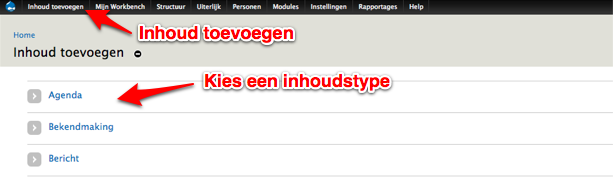
\includegraphics[width=\textwidth]{img/content1.png}
\end{center}

\subsubsection{Content bewerken}\label{contentbewerken}
Algemene werkwijze voor het bewerken van content:
\begin{enumerate}
\item Ga naar het overzicht van alle inhoud: \emph{Mijn Workbench} $\rightarrow$ \emph{Inhoud zoeken}, of ga direct naar \drupalpath{admin/workbench/all-content}.
\item Om de gewenste inhoud sneller te vinden kun je de filterfunctie gebruiken, bovenaan de pagina. Klik bijvoorbeeld bij het label \emph{type} in het lijstje op \emph{Agenda} en vervolgens klik je op \emph{Filteren}. Alleen artikelen van het type \emph{Agenda} zullen nu getoond worden.
\item Zoek naar de titel van het artikel welke je wil gaan bewerken en klik vervolgens op \emph{bewerken} in de meest rechter kolom genaamd \emph{bewerken}.
\item Je bent nu gereed om de content te gaan bewerken. Om de bewerkingen op te slaan klik je onderaan de pagina op de knop \emph{Opslaan}.
\end{enumerate}

\begin{center}
	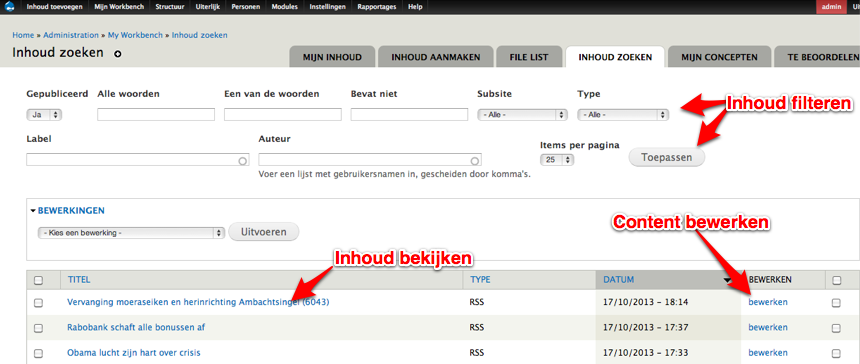
\includegraphics[width=\textwidth]{img/content2.png}
\end{center}

\subsubsection{Content verwijderen}\label{contentverwijderen}
Algemene werkwijze voor het verwijderen van content:
\begin{enumerate}
\item Ga naar het overzicht van alle inhoud: \emph{Mijn Workbench} $\rightarrow$ \emph{Inhoud zoeken}, of ga direct naar \drupalpath{admin/workbench/all-content}.
\item Om de gewenste inhoud sneller te vinden kun je de filterfunctie gebruiken, bovenaan de pagina. Klik bijvoorbeeld bij het label \emph{type} in het lijstje op \emph{Agenda} en vervolgens klik je op \emph{Filteren}. Alleen artikelen van het type \emph{Agenda} zullen nu getoond worden.
\item Zoek naar de titel van het artikel welke je wil gaan bewerken en klik vervolgens op \emph{bewerken} in de meest rechter kolom genaamd \emph{bewerken}.
\item Onderaan de pagina staat de knop \emph{Verwijderen}, klik op deze knop om de content te verwijderen. Na het bevestigen zal de content permanent en onherstelbaar verwijderd worden.
\end{enumerate}

\bigskip

\begin{center}
	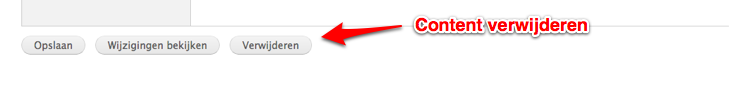
\includegraphics[width=\textwidth]{img/content3.png}
\end{center}

\subsubsection{Content publiceren / goedkeuren}\label{contentpubliceren}
Content publiceren / goedkeuren kan op twee verschillende manieren. Content welke niet is toegevoegd door eindredacteuren moet eerst goedgekeurd worden door een eindredacteur. Content goedkeuren gaat via de \emph{Workflow}\seeone{inhoudgoedkeuren}

Als een eindredacteur zelf content toevoegd kan hij de content ook direct publiceren. Indien je content na het aanmaken direct wilt publiceren, selecteer dan \emph{Gepubliceerd} bij publicatie-opties. 

\begin{center}
	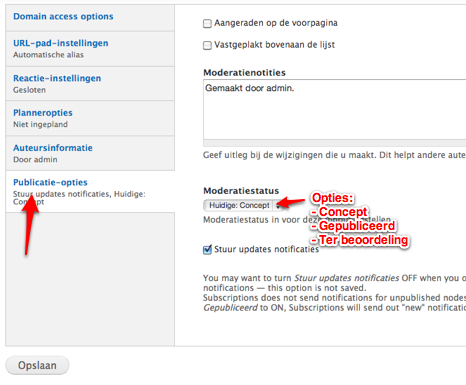
\includegraphics[width=\textwidth]{img/publiceren1.png}
\end{center}
